
%(BEGIN_QUESTION)
% Copyright 2012, Tony R. Kuphaldt, released under the Creative Commons Attribution License (v 1.0)
% This means you may do almost anything with this work of mine, so long as you give me proper credit

Dette hydrostatiske nivåtransmittersystemet er utstyrt med {\it standpipes} og ekstra håndventiler for ``våt kalibrering'' av transmitter:

$$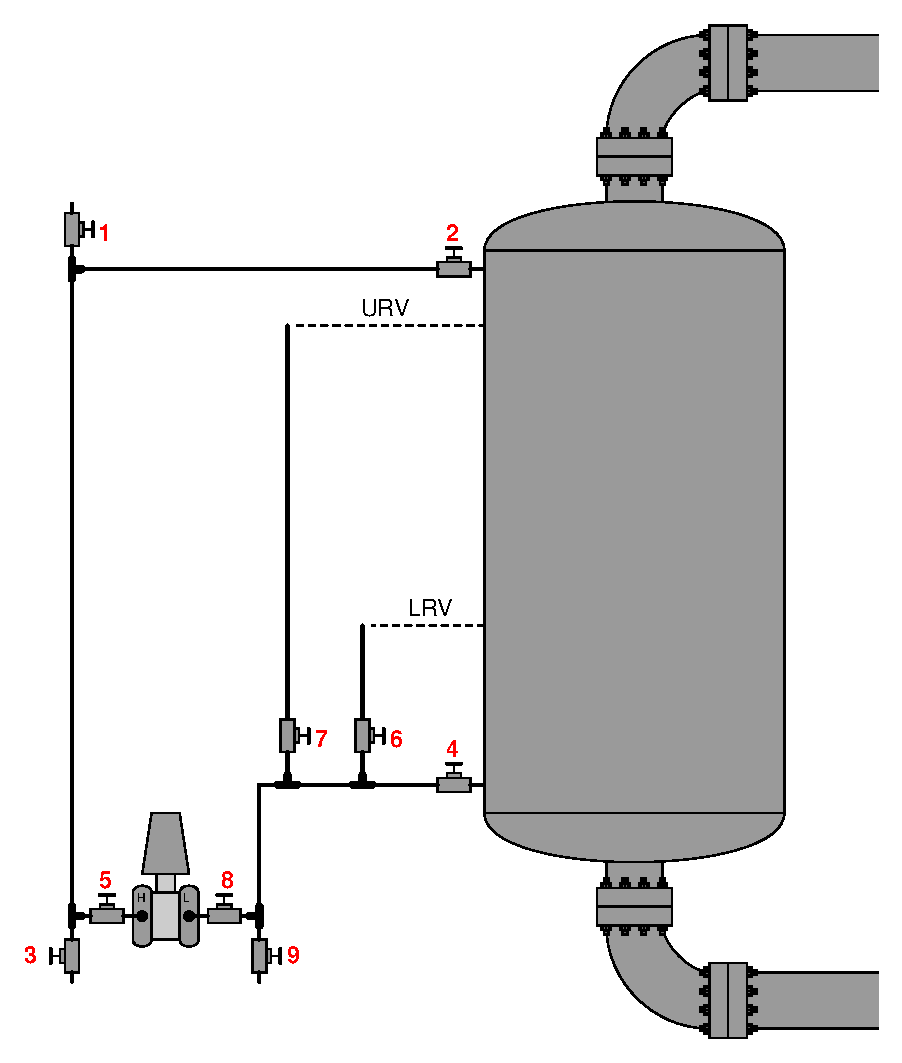
\includegraphics[width=15.5cm]{i01016x01.eps}$$

Identifiser først riktig stilling ({\it åpen} eller {\it stengt}) for hver håndventil i normal drift.

\vskip 10pt

Spesifiser deretter en prosedyre for å påføre LRV ``test pressure'' til transmitteren ved hjelp av ventiler og standpipe.

\underbar{file i01016}
%(END_QUESTION)





%(BEGIN_ANSWER)

Under normal drift:
 
\begin{itemize}
\item{} Åpne ventiler: 2, 4, 5 og 8
\item{} Stengte ventiler: 1, 3, 6, 7 og 9
\end{itemize}

\vskip 10pt

Prosedyre for LRV testtrykk:

\begin{itemize}
\item{} Steng ventil 2 og 4
\item{} Åpne ventil 1 og 6
\item{} Inspiser væskenivå i wet-leg (fyll opp ved behov)
\item{} Åpne ventil 4 litt til væske renner over LRV-standpipe, steng deretter
\item{} {\it Transmitteren ser nå LRV-trykk}
\end{itemize}

%(END_ANSWER)





%(BEGIN_NOTES)



%INDEX% Calibration, generating LRV and URV for hydrostatic transmitter using standpipes
%INDEX% Measurement, level: hydrostatic pressure

%(END_NOTES)

